\chapter{Phương pháp đề xuất}
\label{Chapter3}

\section{Phân loại với mô hình BioMedCLIP và đề xuất cải tiến}
Với việc được tiền huấn luyện trên bộ dữ liệu PMC-15M, đã bao gồm ảnh X-quang, nhóm quyết định sử dụng mô hình BioMedCLIP 
làm mô hình cơ sở để phát triển hệ thống phân loại. Trước tiên, nhóm thực hiện đánh giá khả năng phân loại ảnh 
X-quang xương của mô hình BiomedCLIP \cite{BiomedCLIP} thuần túy để đánh giá khả năng phân loại với một tác vụ riêng biệt
ở miền ảnh X-Quang xương, yêu cầu một độ chính xác cao với độ nhầm lẫn thấp để đáp ứng với yêu cầu thực tế, 
đặc biệt là trong lĩnh vực y khoa.

Bộ dữ liệu được sử dụng để đánh giá là BTXRD, gồm tổng cộng 3.746 hình ảnh, trong đó phân bổ 
thành 1.879 ảnh xương bình thường, 1.525 ảnh u xương lành tính và 342 ảnh u xương ác tính.

\subsection{Quá trình phân loại của mô hình BiomedCLIP}
Mô hình BiomedCLIP gốc trong thiết lập \textit{zero-shot} thực hiện quá trình phân loại dựa trên cơ chế đối sánh 
Hình ảnh - Văn bản (Vision-Language Matching) thay vì sử dụng các lớp phân loại (classification head) truyền thống. 
Quy trình này bao gồm 5 bước cốt lõi sau:

\begin{enumerate}
    \item \textbf{Xây dựng bộ mô tả văn bản (Text Prompting):} Các nhãn phân loại rời rạc được chuyển đổi thành các câu lệnh mang ngữ nghĩa lâm sàng phong phú nhằm cung cấp thông tin ngữ cảnh cho mô hình (Ví dụ: "A radiograph showing {tên\_bệnh\_lý}").
    \item \textbf{Trích xuất đặc trưng văn bản (Text Encoding):} Các câu mô tả được đưa qua nhánh \textit{Text Encoder} (kiến trúc PubMedBERT) để chuyển đổi thành các vector đặc trưng văn bản (\textit{text embeddings}) trong không gian biểu diễn chung.
    \item \textbf{Trích xuất đặc trưng hình ảnh (Image Encoding):} Ảnh X-quang đầu vào được xử lý qua nhánh \textit{Vision Encoder} (kiến trúc Vision Transformer - ViT) để trích xuất vector đặc trưng hình ảnh (\textit{image embedding}) đại diện cho các thông tin thị giác.
    \item \textbf{Tính toán độ tương đồng (Cosine Similarity):} Mô hình tiến hành đo lường khoảng cách giữa vector hình ảnh với tất cả các vector văn bản thông qua phép toán độ tương đồng Cosine. Cặp ảnh - văn bản có sự tương hợp cao nhất về mặt ngữ nghĩa y khoa sẽ đạt điểm số lớn nhất.
    \item \textbf{Đưa ra dự đoán cuối cùng:} Các điểm số tương đồng được chuẩn hóa thông qua hàm Softmax để chuyển thành phân phối xác suất. Lớp tương ứng với câu mô tả có xác suất cao nhất sẽ được lựa chọn làm kết quả dự đoán của mô hình.
\end{enumerate}

\subsection{Kết quả phân loại}

\begin{table}[htbp]
\centering
\caption{Các chỉ số đánh giá tổng quan (Aggregated/Macro)}
\label{tab:macro_metrics}
\begin{tabular}{|l|c|}
\hline
\textbf{Chỉ số (Metric)} & \textbf{Giá trị} \\
\hline
Độ chính xác (Accuracy) & 0.3381 \\
F1 Macro & 0.1056 \\
AUROC Macro & 0.5773 \\
Độ nhạy (Sensitivity Macro) & 0.1499 \\
Độ đặc hiệu (Specificity Macro) & 0.9064 \\
Độ chuẩn xác (Precision Macro) & 0.1123 \\
\hline
\end{tabular}
\end{table}


\begin{itemize}
    \item \textbf{Độ đặc hiệu cao (Specificity = 0.9064):} Mô hình làm rất tốt việc \textit{loại trừ}. Nghĩa là khi nó dự đoán một ca là "không mắc bệnh" (âm tính), thì khả năng cao là bệnh nhân thực sự không mắc bệnh.
    \item \textbf{Độ nhạy cực thấp (Sensitivity = 0.1499):} Đây là "báo động đỏ" trong y tế. Độ nhạy chỉ đạt $\sim$15\% có nghĩa là mô hình \textbf{bỏ sót tới 85\% các ca thực sự có khối u} (Âm tính giả - False Negative cao). Mô hình đang có xu hướng an toàn là dự đoán mọi thứ thành lớp Bình thường (Normal).
    \item \textbf{Độ chuẩn xác (Precision = 0.1123) và F1 Macro (0.1056) rất thấp:} Khi mô hình quyết định cảnh báo một ca là khối u, thì phần lớn các cảnh báo đó là sai (Dương tính giả - False Positive cao). F1 Macro thấp ($\sim$10.5\%) cho thấy mô hình xử lý cực kỳ kém trên toàn bộ các lớp.
    \item \textbf{Độ chính xác tổng (Accuracy = 0.3381):} Chỉ có khoảng 33.8\% tổng số mẫu được dự đoán đúng. Tuy nhiên, trong y tế, Accuracy là một chỉ số "đánh lừa" nếu dữ liệu bị mất cân bằng.
    \item \textbf{AUROC Macro (0.5773):} Chỉ số này nhỉnh hơn mức độ đoán mò (0.5) một chút. Nó chứng tỏ mô hình BiomedCLIP gốc chưa có đủ khả năng phân biệt (discrimination) rõ ràng giữa các ranh giới của các loại u xương.
\end{itemize}

\begin{table}[htbp]
\centering
\caption{Chỉ số F1 (F1-score) chi tiết theo từng lớp}
\label{tab:f1_per_class}
\begin{tabular}{|l|c|}
\hline
\textbf{Lớp chẩn đoán (Class)} & \textbf{F1-Score} \\
\hline
Normal (Bình thường) & 0.5790 \\
Simple bone cyst (Nang xương đơn giản) & 0.1935 \\
Osteosarcoma (Sarcoma xương) & 0.1250 \\
Giant cell tumor (U tế bào khổng lồ) & 0.1212 \\
Osteofibroma (U xơ xương) & 0.0375 \\
Osteochondroma (U sụn xương) & 0.0000 \\
Multiple osteochondromas (Đa u sụn xương) & 0.0000 \\
Other bt (U lành tính khác) & 0.0000 \\
Synovial osteochondroma (U sụn màng hoạt dịch) & 0.0000 \\
Other mt (U ác tính khác) & 0.0000 \\
\hline
\end{tabular}
\end{table}

Bảng F1-Score \ref{tab:f1_per_class} từng lớp chính là minh chứng rõ ràng nhất cho tình trạng \textbf{mất cân bằng dữ liệu (data imbalance)}:
\begin{itemize}
    \item \textbf{Lớp Normal (0.5790):} Là lớp có kết quả cao nhất. Điều này dễ hiểu vì dữ liệu y tế luôn có số lượng ảnh bình thường áp đảo. Mô hình đã học được "thiên kiến" (bias), dẫn đến việc dự đoán ưu tiên lớp này để tối ưu Accuracy tổng.
    \item \textbf{Các lớp có số liệu thấp (Osteosarcoma, Giant cell tumor, Simple bone cyst):} Chỉ đạt mức F1 từ 0.12 đến 0.19. Dù Sarcoma xương (Osteosarcoma) là một bệnh lý có đặc điểm hình ảnh khá đặc trưng, mô hình zero-shot vẫn gặp khó khăn trong việc nhận diện chính xác.
    \item \textbf{Các lớp bị điểm 0 tuyệt đối (Osteochondroma, Synovial osteochondroma, \dots):} Mô hình hoàn toàn "mù" trước các lớp này (không đoán trúng được ca nào). Điều này xảy ra khi đặc trưng hình ảnh của các khối u này quá hiếm hoặc quá phức tạp để mô hình gốc có thể nội suy ra được mà không qua quá trình huấn luyện (fine-tuning).
\end{itemize}


\subsection{Kết luận}
    Các kết quả này chỉ ra ba hạn chế chính của mô hình:
        \begin{enumerate}
            \item Khoảng cách miền giữa dữ liệu tiền huấn luyện và ảnh X-quang xương;
            \item Thiếu thông tin ngữ cảnh lâm sàng khi mô hình gốc gần như chỉ sử dụng ảnh;
            \item Chưa xử lý được đặc tính đa nhãn, mất cân bằng dữ liệu của bài toán.
        \end{enumerate}
    Do đó, việc tinh chỉnh lại mô hình để cải hiện hiệu năng, giảm khoảng cách miền và đáp ứng bài toán thiếu hụt dữ liệu là cần thiết, 
    nghiên cứu đề xuất một kiến trúc đa phương thức gồm hai giai đoạn huấn luyện:
    \begin{enumerate}
        \item Thích nghi miền dựa trên LoRA để các vector đặc trưng mang tính khả tách.
        \item Hợp nhất ảnh–văn bản bằng cơ chế chú ý chéo hai chiều và học phân loại đa nhãn dựa trên mạng nguyên mẫu.
    \end{enumerate}
    Các cải tiến cụ thể hơn sẽ được trình bày trong phần tiếp theo.

\subsection{Đề xuất cải tiến}
Dựa trên những hạn chế của mô hình gốc, nghiên cứu đề xuất các thay đổi quan trọng sau:

\textbf{Lựa chọn cách finetuning với đặc thù ít dữ liệu:}
LoRA được lựa chọn vì đây là phương pháp tinh chỉnh hiệu quả về tham số, cho phép thích nghi BioMedCLIP với miền ảnh X-quang xương 
mà vẫn bảo toàn tri thức tiền huấn luyện. So với tinh chỉnh toàn bộ tham số, LoRA giảm nguy cơ quá khớp dữ liệu và quên thảm khốc 
trong bối cảnh dữ liệu y khoa có quy mô hạn chế và phân phối mất cân bằng.
Mặc dù nghiên cứu sử dụng toàn bộ dữ liệu hiện có, nhiều lớp vẫn chỉ chứa số lượng mẫu rất ít. 
Do đó, bài toán ở cấp độ từng lớp mang đặc tính học ít mẫu, và LoRA giúp hệ thống duy trì khả năng thích nghi tốt trong các trường hợp 
này.

\textbf{Lựa chọn mục tiêu huấn luyện cho học biểu diễn:}
Loss tương phản gốc của BioMedCLIP (InfoNCE) giả định quan hệ một-một giữa ảnh và văn bản, 
do đó chưa phù hợp với dữ liệu X-quang xương, nơi một ảnh có thể tương ứng với nhiều mô tả ngữ nghĩa và nhiều nhãn đồng thời.
Vì vậy, nghiên cứu thay thế hàm mất mát tương phản bằng hàm mất mát tương ứng ngữ nghĩa (Semantic Matching Loss) 
nhằm khai thác mức độ tương đồng ngữ nghĩa 
giữa ảnh và văn bản, giảm ảnh hưởng của các cặp âm tính giả và hỗ trợ tốt hơn cho bài toán đa nhãn. 
Tuy nhiên, Semantic Matching Loss không trực tiếp xử lý mất cân bằng dữ liệu. Do đó, ở giai đoạn phân loại đa nhãn, 
nghiên cứu kết hợp thêm các hàm mất mát chuyên biệt như hàm mất mát không đối xứng (Asymmetric Loss) 
để tăng khả năng nhận diện các lớp hiếm.

\textbf{Xử lý đa nhãn và mất cân bằng dữ liệu trong học phân loại:}
Do bài toán được xây dựng theo hướng phân loại đa nhãn với dữ liệu mất cân bằng nghiêm trọng, 
hàm mất mát Cross-Entropy không còn phù hợp vì giả định các lớp loại trừ lẫn nhau. 
Nghiên cứu sử dụng kiến trúc mạng nguyên mẫu (Prototypical Network) dạng tham số (Parametric Prototypical Network) 
kết hợp với hàm mất mát không đối xứng nhằm tối ưu hiệu suất trên các lớp hiếm.

\textbf{Phát hiện OOD (Out-of-Distribution):}
Việc phát hiện dữ liệu ngoài phân phối (OOD) được thực hiện dựa trên khoảng cách Cosine giữa các đặc trưng và các nguyên mẫu (prototypes) trong không gian biểu diễn chung,
thay vì xác suất Softmax. Mô hình có thể được huấn luyện chỉ với dữ liệu trong phân phối, và sau đó nếu có dữ liệu OOD, 
có thể mở rộng bằng cách bổ sung hàm mất mát OOD Margin Loss để ép các mẫu ngoài phân phối nằm xa tất cả các nguyên mẫu, 
tăng khả năng phân biệt dữ liệu bất thường.

\section{Ý tưởng ban đầu} 

Dựa trên các nghiên cứu liên quan, nhóm đề xuất xây dựng một hệ thống học sâu đa phương thức nhằm khai thác đồng thời thông tin từ ảnh X-quang và dữ liệu lâm sàng văn bản. Đặc biệt, hệ thống được thiết kế theo hướng tích hợp tri thức y khoa nhằm nâng cao khả năng học ít mẫu và phát hiện dữ liệu ngoài phân phối. Cụ thể, kiến trúc bao gồm các thành phần chính như sau:
    \begin{itemize}
        \item \textbf{Bộ mã hóa ảnh:} Kế thừa lại mô hình ViT-Base của phương pháp BiomedCLIP \cite{BiomedCLIP}
        \item \textbf{Bộ mã hóa văn bản:} Kế thừa lại mô hình PubMedBERT của phương pháp BiomedCLIP \cite{BiomedCLIP}
        \item \textbf{Bộ dung hợp dữ liệu:} Kỹ thuật Bidirectional Cross-Attention được xây dựng dựa trên cơ chế cross-attention 
        nhằm học mối quan hệ ngữ nghĩa giữa đặc trưng hình ảnh và đặc trưng văn bản y khoa.
        \item \textbf{Bộ phân loại:} Dùng phương pháp metric-based few-shot learning với một prototypical network, 
        nhãn được quyết định bởi khoảng cách đến các prototype trong không gian biểu diễn chung, 
        thay vì lớp phân loại truyền thống làm ràng buộc mô hình phân loại vào các nhãn đã biết, 
        giúp phát hiện dữ liệu ngoài phân phối khi khoảng cách đó vượt quá ngưỡng xác định.

    \end{itemize}
    Đồng thời, các trọng số attention và thông tin từ tri thức y khoa được khai thác để trực quan hóa và giải thích kết quả dự đoán.

\section{Giai đoạn off-line}
Giai đoạn off-line nhằm xây dựng bộ tham số cho mô hình, thiết lập không gian biểu diễn chung và học cách dung hợp giữa đặc trưng hình ảnh X-quang và ngữ nghĩa y khoa.

Giai đoạn off-line gồm 2 công đoạn: Domain-Adaption và Fine-tuning. 
Trong đó, công đoạn Domain-Adaption nhằm mục đích giúp mô hình thích nghi từ miền dữ liệu tiền huấn luyện lớn sang miền dữ liệu y khoa đích của bài toán, 
trong khi công đoạn Fine-tuning tập trung vào việc tối ưu hóa khả năng dung hợp dữ liệu 
và phân loại trên tập dữ liệu mục tiêu.

\subsection{Domain-Adaption với kỹ thuật LoRA}
\begin{figure}[H]
    \centering
    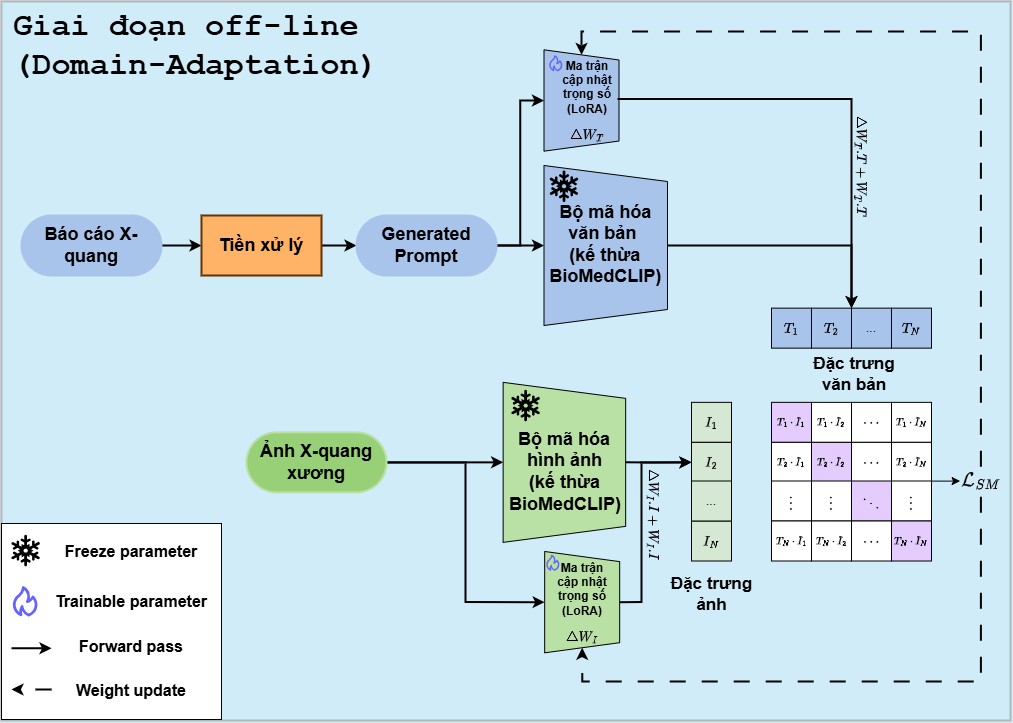
\includegraphics[width=1\linewidth]{images/domain-adaption.png}
    \caption{Sơ đồ chung của hệ thống trong công đoạn Domain-Adaption.}
    \label{fig:domain-adaption}
\end{figure}

Trong công đoạn này, mục tiêu chính giúp mô hình học cách biểu diễn sao cho các cặp ảnh và báo cáo ảnh X-Quang 
nằm gần nhau hơn trong không gian biểu diễn bằng cách tối ưu hàm mất mát khớp ngữ nghĩa (Semantic Matching Loss), 
mô hình tuân theo framework contrastive learning để căn chỉnh bộ mã hóa BiomedCLIP về miền dữ liệu X-Quang xương được sử dụng, 
với đầu vào là các cặp ảnh X-quang và phân tích ảnh tương ứng của bác sĩ. Dữ liệu được đưa vào bộ mã hóa tương ứng để trích xuất đặc trưng, 
sau đó được chiếu vào không gian chung và chuẩn hóa để so sánh và thực hiện điều chỉnh. 
Kết quả là các cặp hình ảnh và văn bản giống nhau hoặc chung lớp nằm gần nhau hơn gọi là các semantic clusters, 
trong khi các cặp văn bản khác lớp sẽ nằm xa nhau hơn.

Nhóm thực hiện tinh chỉnh (fine-tuning) đồng thời Vision Encoder và Text Encoder bằng kỹ thuật LoRA (Low-Rank Adaptation). 
LoRA được lựa chọn vì đây là phương pháp tinh chỉnh hiệu quả về tham số, 
cho phép thích nghi BioMedCLIP với miền ảnh X-quang xương mà vẫn bảo toàn tri thức tiền huấn luyện. 

Mặc dù nghiên cứu sử dụng toàn bộ dữ liệu hiện có, nhiều lớp vẫn chỉ chứa số lượng mẫu rất ít. Do đó, bài toán ở cấp độ từng lớp mang đặc tính few-shot, và LoRA giúp hệ thống duy trì khả năng thích nghi tốt trong các trường hợp này. Nghiên cứu lựa chọn LoRA thay vì QLoRA vì mục tiêu chính là thích nghi miền hiệu quả trong điều kiện dữ liệu hạn chế, thay vì tối ưu bộ nhớ cho các mô hình siêu lớn. BioMedCLIP có quy mô tham số vừa phải, cho phép huấn luyện hiệu quả với LoRA trên phần cứng hiện có mà không cần lượng tử hóa. Ngoài ra, việc giữ nguyên trọng số ở độ chính xác đầy đủ giúp bảo toàn các đặc trưng hình ảnh tinh vi của ảnh X-quang xương, vốn rất quan trọng đối với việc nhận diện các tổn thương nhỏ và các lớp hiếm.
    
    Để cập nhật trọng số của ma trận LoRA, nhóm sử dụng \textbf{Hàm mất mát Khớp ngữ nghĩa (Semantic Matching Loss - $\mathcal{L}_{SM}$)} nhằm đồng bộ hóa không gian biểu diễn đa phương thức. Loss tương phản gốc của BioMedCLIP (InfoNCE) giả định quan hệ một-một giữa ảnh và văn bản, do đó chưa phù hợp với dữ liệu X-quang xương, nơi một ảnh có thể tương ứng với nhiều mô tả ngữ nghĩa và nhiều nhãn đồng thời.
    
    Vì vậy, nghiên cứu thay thế contrastive loss bằng Semantic Matching Loss nhằm khai thác mức độ tương đồng ngữ nghĩa giữa ảnh và văn bản, giảm ảnh hưởng của các cặp âm tính giả và hỗ trợ tốt hơn cho bài toán đa nhãn. Tuy nhiên, Semantic Matching Loss không trực tiếp xử lý mất cân bằng dữ liệu. Do đó, ở giai đoạn phân loại đa nhãn, nghiên cứu kết hợp thêm các hàm mất mát chuyên biệt như Asymmetric Loss để tăng khả năng nhận diện các lớp hiếm.

    Mức độ tương đồng Cosine giữa đặc trưng ảnh $z_i^I$ và đặc trưng văn bản $z_j^T$:
    \begin{equation}
    \operatorname{sim}(z_i^I, z_j^T) = \frac{z_i^I \cdot z_j^T}{\|z_i^I\| \|z_j^T\|}
    \end{equation}

    Hàm mất mát được sử dụng là Semantic Matching Loss $\mathcal{L}_{\mathrm{SM}}$ được định nghĩa dựa trên ma trận mục tiêu mềm $s_{ij}$:
    \begin{equation}
    \mathcal{L}_{\mathrm{SM}} = -\frac{1}{N} \sum_{i=1}^{N} \sum_{j=1}^{N} s_{ij} \log \frac{\exp\left(\operatorname{sim}(z_i^I,z_j^T)/\tau\right)}{\sum_{k=1}^{N} \exp\left(\operatorname{sim}(z_i^I,z_k^T)/\tau\right)}
    \end{equation}
    trong đó, $N$ là kích thước mini-batch, $s_{ij}$ là ma trận mục tiêu xác định các mẫu chung lớp, và $\tau$ là siêu tham số nhiệt độ (temperature) giúp điều chỉnh độ nhạy của hàm phạt đối với các mẫu âm tính (negative samples). Bằng cách tối ưu $\mathcal{L}_{SM}$, mô hình đẩy các đặc trưng giải phẫu X-quang cục bộ hội tụ chặt chẽ về đúng định nghĩa y khoa của chúng trong không gian chung.

Công đoạn Domain-Adaption giúp mô hình học cách biểu diễn sao cho các cặp ảnh và báo cáo khám tổng quát chung lớp nằm gần nhau hơn trong không gian biểu diễn, 
Semantic Matching Loss giúp các dữ liệu chung lớp nằm gần nhau thay vì ràng buộc như contrastive learning truyền thống rằng 
các cặp ảnh và báo cáo chung lớp dù không tương ứng dù nằm chung lớp vẫn phải nằm cách xa nhau ra. 
Điều này cực quan trọng với bài toán dữ liệu còn hạn chế, giúp tránh trường hợp dữ liệu nằm chung nhóm không hội tụ. 
Trong quá trình huấn luyện, đạo hàm từ hàm mất mát $\mathcal{L}_{SM}$ chỉ chảy qua và cập nhật ma trận 
$A \in \mathrm{R}^{r \times k}$ và $B \in \mathrm{R}^{d \times r}$ (với hạng $r \ll \min(d, k)$) của LoRA. 
Tổng số tham số cần học (learnable parameters) chiếm dưới 5\% toàn mạng.


\subsection{Fusion-learning}
\begin{figure}[H]
    \centering
    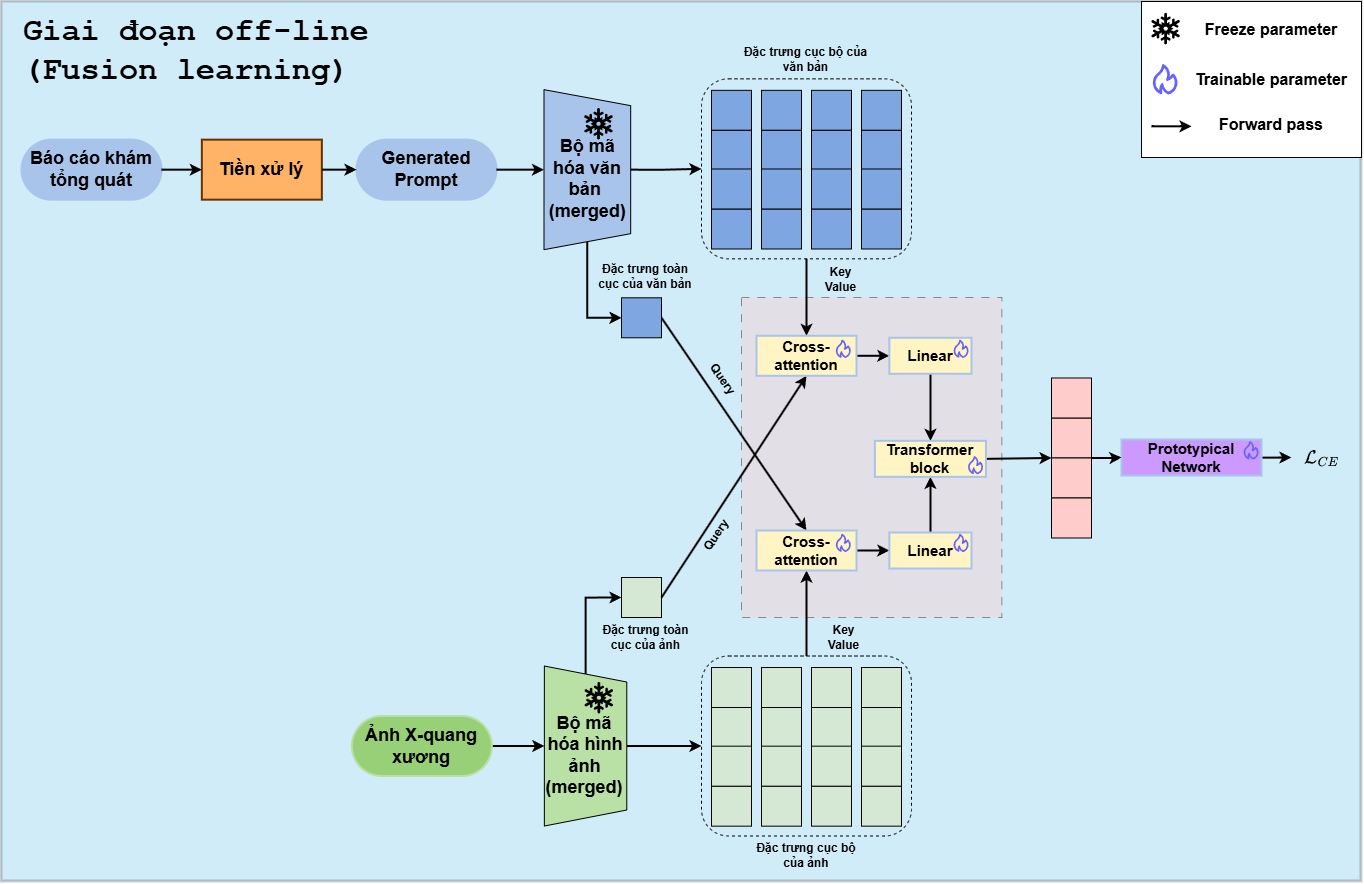
\includegraphics[width=1\linewidth]{images/fusion-learning.png}
    \caption{Sơ đồ chung của hệ thống trong công đoạn Fusion-learning.}
    \label{fig:fusion-learning}
\end{figure}
Trong công đoạn này, nhóm tối ưu khả năng khai thác và dung hợp dữ liệu bằng cách sử dụng kỹ thuật Bidirectional Cross-Attention để học các mối liên hệ giữa đặc trưng đặc trưng toàn cục của ảnh X-Quang với đặc trưng cục bộ của báo cáo khám tổng quát và ngược lại.

Để mô phỏng sát với quá trình học phân tích ảnh thực tế của bác sĩ, dữ liệu đầu vào của công đoạn này là các cặp ảnh X-quang và báo cáo khám tổng quát. Các dữ liệu này được đưa vào bộ mã hóa tương ứng để trích xuất đặc trưng. 
Kỹ thuật cross-attention được sử dụng để học các mối liên hệ giữa các đặc trưng này. Đặc trưng toàn cục của ảnh X-quang được sử dụng để tìm các đặc trưng cục bộ của báo cáo khám tổng quát có liên quan và ngược lại, 
đặc trưng toàn cục của văn bản được sử dụng để tìm các đặc trưng cục bộ của ảnh X-quang có liên quan. Sau đó, các đặc trưng có liên quan được đưa vào một khối Transformer, 
nơi chúng được kết hợp một lần nữa thông qua cơ chế attention để học sự phụ thuộc giữa các đặc trưng, tương quan ngữ nghĩa ở mức độ sâu hơn
 trước khi được đưa vào bộ phân loại cuối cùng để dự đoán nhãn bệnh lý. Sự khác biệt của dự đoán với nhãn thực tế sẽ được tính toán
  và sử dụng để cập nhật tham số của các khối Cross-Attention, Linear Projection và Transformer cũng như Classifier.

Do bài toán được xây dựng theo hướng phân loại đa nhãn với dữ liệu mất cân bằng nghiêm trọng, hàm mất mát Cross-Entropy không còn phù hợp vì giả định các lớp loại trừ lẫn nhau. Nghiên cứu sử dụng kiến trúc Prototypical Network dạng tham số (Parametric Prototypical Network) kết hợp với hàm mất mát Asymmetric Loss nhằm tối ưu hiệu suất trên các lớp hiếm.

\begin{figure}[H]
    \centering
    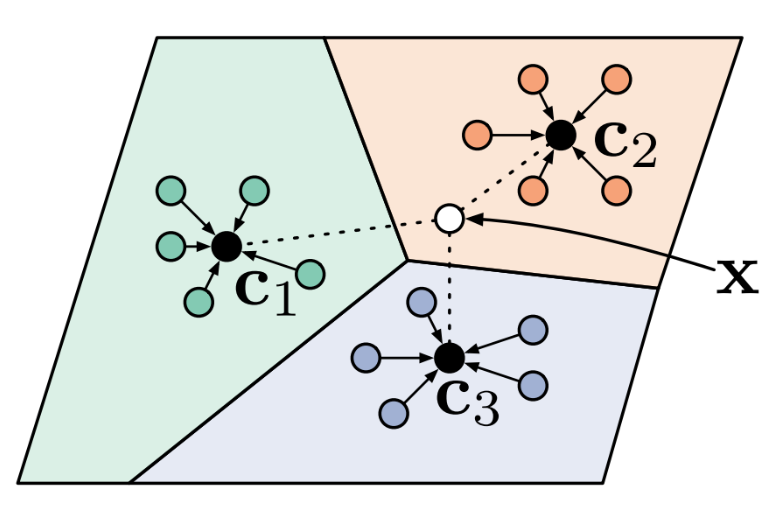
\includegraphics[width=1\linewidth]{images/prototypical_network.png}
    \caption{Sơ đồ mạng prototypical.}
    \label{fig:prototypical-network}
\end{figure}

Thay vì tính toán giá trị prototype cố định bằng trung bình cộng của các mẫu hỗ trợ, các prototype lớp $c_k$ được định nghĩa là các vector trọng số có thể học được (learnable parameters) và được cập nhật trực tiếp qua quá trình lan truyền ngược (backpropagation). 
Khoảng cách giữa embedding hợp nhất $z_i$ và các prototype $c_k$ được sử dụng để đưa ra dự đoán đa nhãn, đồng thời hỗ trợ phát hiện dữ liệu ngoài phân phối thông qua ngưỡng khoảng cách đến prototype gần nhất. Nghiên cứu sử dụng khoảng cách Cosine (Cosine Distance) giữa đặc trưng đã chuẩn hóa L2 để đảm bảo sự ổn định trong không gian nhúng của mô hình đa phương thức:
\begin{equation}
d(z_i, c_k) = 1 - \frac{z_i \cdot c_k}{\|z_i\|_2 \|c_k\|_2}
\end{equation}

Mức độ tương đồng Cosine có trọng số tỷ lệ $\tau$ được tính để xác định xác suất dự đoán của mẫu $i$ đối với lớp $k$ bằng hàm Sigmoid:
\begin{equation}
p_{ik} = \sigma\left(\tau (1 - d(z_i, c_k))\right)
\end{equation}

Hàm mất mát chính trong giai đoạn này là Asymmetric Loss (ASL) nhằm xử lý đa nhãn và mất cân bằng dữ liệu bằng cách điều chỉnh hệ số suy giảm $\gamma$ khác nhau cho nhãn dương và nhãn âm:
\begin{equation}
\mathcal{L}_{\mathrm{ASL}} = -\frac{1}{N} \sum_{i=1}^{N} \sum_{k=1}^{K} \left[ y_{ik}(1-p_{ik})^{\gamma^+}\log(p_{ik}) + (1-y_{ik})p_{m,ik}^{\gamma^-}\log(1-p_{m,ik}) \right]
\end{equation}
với $p_{m,ik} = \max(0, p_{ik} - \text{clip})$ là xác suất đã dịch chuyển nhằm loại bỏ các mẫu âm tính có độ tin cậy cao.

Ngoài ra, hàm Prototype Loss $\mathcal{L}_{\mathrm{proto}}$ được áp dụng để kéo đặc trưng gần với prototype lớp tương ứng và đẩy ra xa khỏi các prototype lớp khác:
\begin{equation}
\mathcal{L}_{\mathrm{proto}} = \frac{1}{N} \sum_{i=1}^{N} \sum_{k=1}^{K} \left[ y_{ik}d(z_i,c_k) + (1-y_{ik}) \max(0,\delta-d(z_i,c_k)) \right]
\end{equation}

Việc phát hiện dữ liệu ngoài phân phối (OOD) được thực hiện dựa trên khoảng cách Cosine giữa embedding và các prototype. Do đặc thù dữ liệu y khoa khó thu thập mẫu OOD đại diện, mô hình có thể được huấn luyện chỉ với dữ liệu trong phân phối. Nếu có dữ liệu OOD, có thể mở rộng mô hình bằng cách bổ sung hàm mất mát OOD Margin Loss $\mathcal{L}_{\mathrm{OOD}}$ để ép các mẫu ngoài phân phối nằm xa tất cả các prototype:
\begin{equation}
\mathcal{L}_{\mathrm{OOD}} = \frac{1}{N_{\mathrm{OOD}}} \sum_{i=1}^{N_{\mathrm{OOD}}} \max \left( 0, m_{\mathrm{OOD}} - \min_k d(z_i^{\mathrm{OOD}},c_k) \right)
\end{equation}

Tổng hợp lại, hàm mất mát cho giai đoạn học phân loại được định nghĩa như sau:
\begin{equation}
\mathcal{L} = \mathcal{L}_{\mathrm{ASL}} + \lambda_1 \mathcal{L}_{\mathrm{proto}} + \lambda_2 \mathcal{L}_{\mathrm{OOD}}
\end{equation}
Bằng cách tối ưu tổ hợp hàm mất mát này, mô hình học được cách phân loại chính xác các bệnh lý xương khớp dưới dạng đa nhãn, cải thiện năng lực dự đoán trên các lớp hiếm và cung cấp khả năng phát hiện mẫu bệnh lý bất thường (OOD).

\section{Giai đoạn online}
\begin{figure}[H]
    \centering
    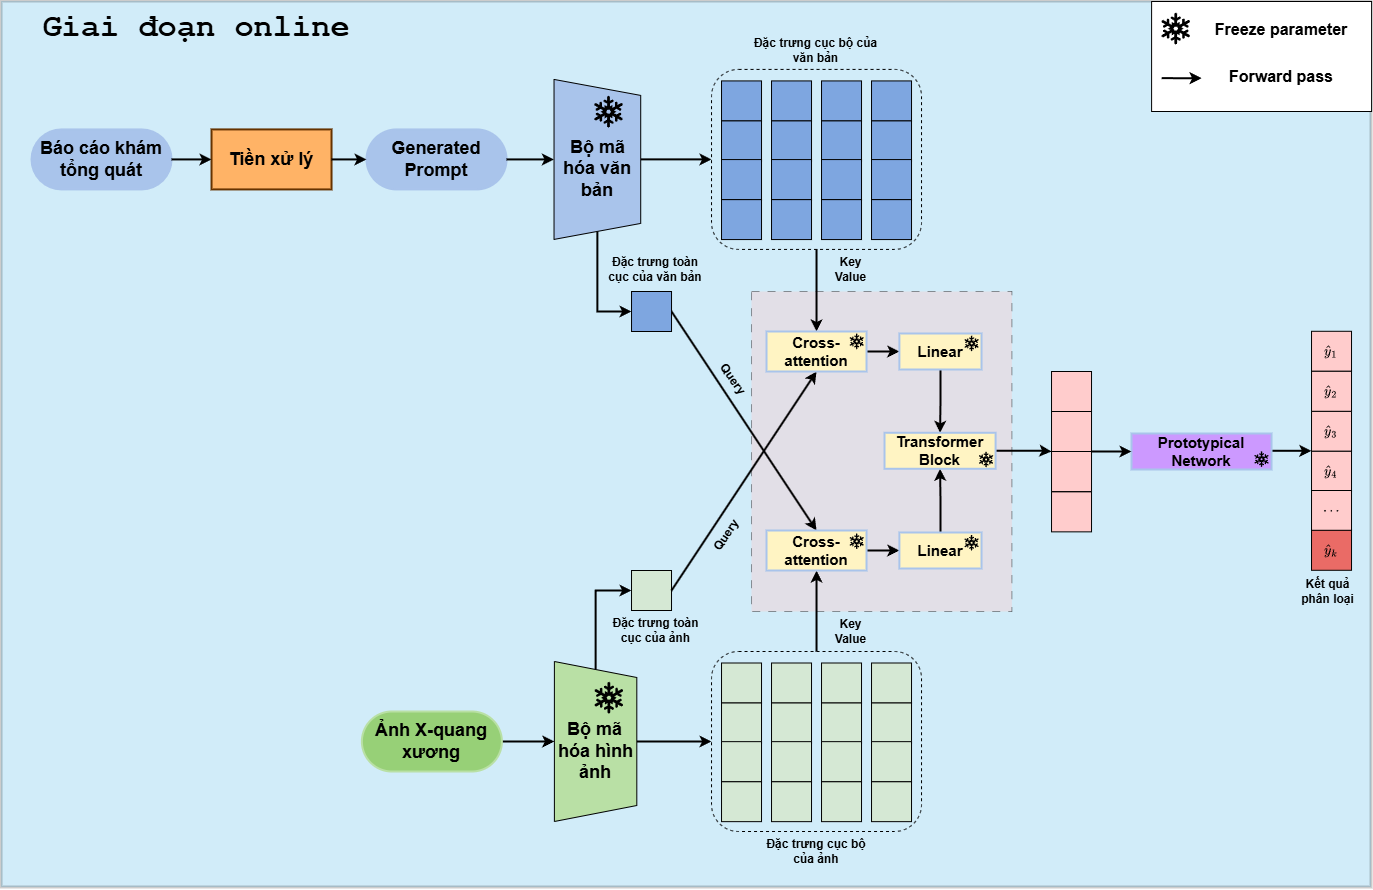
\includegraphics[width=1\linewidth]{images/online.png}
    \caption{Sơ đồ chung của hệ thống trong giai đoạn online.}
    \label{fig:online}
\end{figure}

Sơ đồ của hệ thống trong giai đoạn online được trình bày trong Hình \ref{fig:online}. Gần tương ứng với công đoạn Fine-tuning, 
ảnh X-Quang cùng báo cáo tổng quát gồm lời khai của bệnh nhân và tiền sử bệnh lý sau tiền xử lí được đưa vào bộ mã hóa tương ứng để trích xuất đặc trưng.
Các đặc trưng này được đưa vào khối Cross-Attention để học các mối liên hệ tương tác giữa đặc trưng toàn cục với các đặc trưng cục bộ, 
sau đó được đưa vào khối Transformer để hợp nhất đặc trưng đa phương thức ở mức độ sâu hơn trước khi được đưa vào mạng prototypical để dự đoán nhãn bệnh lý, 
ở đây, nhãn được lựa chọn dựa trên khoảng cách đến các prototype, nếu khoảng cách đến prototype gần nhất vượt quá ngưỡng nhất định, mô hình sẽ đánh dấu là không chắc chắn.
Ngoài ra, các trọng số attention và thông tin từ tri thức y khoa được khai thác để trực quan hóa và giải thích kết quả dự đoán. 
Cụ thể, mô hình có thể tạo ra các bản đồ nhiệt trực quan hóa trên ảnh X-quang dựa trên các trọng số attention để giải thích dự đoán của mô hình.

\section{Đóng góp của phương pháp}
\begin{itemize}
    \item \textbf{Tích hợp tri thức y khoa với biểu diễn đa phương thức:} Không chỉ sử dụng kết hợp cả hai phương thức dữ liệu, 
    phương pháp đã thực hiện trích xuất các thông tin cần thiết từ văn bản y khoa theo khuôn mẫu, giúp giảm nhiễu ngôn ngữ tự nhiên, tăng tính nhất quán ngữ nghĩa; 
    đồng thời việc làm giàu tri thức qua UMLS giúp làm giàu ngữ nghĩa văn bản theo chuẩn y khoa mà không gặp vấn đề hallucination so với việc tạo ra mô tả bằng LLM.
    \item \textbf{Cơ chế Cross-Attention có hướng dẫn tri thức:} Việc sử dụng cơ chế Cross-Attention có hướng dẫn tri thức giúp mô hình tập trung vào các vùng ảnh có liên quan đến bệnh lý, 
    thay vì các vùng nền không liên quan. Điều này không chỉ cải thiện hiệu năng mà còn cung cấp khả năng giải thích thông qua việc truy vết mối liên hệ giữa khái niệm y khoa và vùng ảnh được chú ý.
    \item \textbf{Cơ chế fusion ở nhiều cấp độ:} Việc kết hợp đặc trưng toàn cục và cục bộ thông qua Cross-Attention và khối Transformer giúp mô hình khai thác tối đa dữ liệu 
    và học được các mối liên hệ phức tạp giữa hai nguồn dữ liệu, từ đó cải thiện hiệu suất phân loại và khả năng giải thích của mô hình.
    \item \textbf{Giảm nguy cơ suy giảm không gian ngữ nghĩa trong bối cảnh dữ liệu hạn chế:} 
Cơ chế cập nhật tham số bằng LoRA giúp các bộ mã hóa thích nghi với dữ liệu y khoa đích mà không làm mất mát các tri thức đã học. Điều này giúp hạn chế hiện tượng overfitting và giảm độ phức tạp tính toán.
    \item \textbf{Cơ chế phát hiện dữ liệu ngoài phân phối:} Mô hình có khả năng phát hiện dữ liệu ngoài phân phối với mạng prototypical.
\end{itemize}
